\chapter{Corpos Finitos}
\label{cha:corpos-finitos}

Um {\em corpo} é uma estrutura matemática formada por um conjunto $F$ e duas operações ($+$ e $\cdot$) tal que:
\begin{itemize}
\item Os elementos de $F$ formam um grupo\footnote{Ver capítulo \ref{cha:criptografia-assimetrica}} com a operação $+$ e o elemento neutro é o $0$.
\item Os elementos de $F$, com exceção do $0$, formam um grupo com a operação $\cdot$ e o elemento neutro é o $1$.
\item Para todo $a, b, c \in F$ temos que $a \cdot(b + c) = a \cdot b + a \cdot c$ (distributividade).
\end{itemize}
 
O conjunto dos números reais com as operações convencionais de soma e multiplicação é um corpo.

Estamos interessados, porém, em corpos finitos, também conhecidos como {\em corpos de Galois}.
Um teorema interessante, mas cuja demonstração foge ao escopo dessas notas, estabelece que a cardinalidade de um corpo finito é necessariamente uma potência de um primo.
Em símbolos, se $\langle F, +, \cdot \rangle$ é um corpo então $|F| = p^m$ em que $p$ é um número primo e $m$ um inteiro.

Vamos representar por $GF(p)$ o corpo definido pelo conjunto $\mathbb{Z}_p$ e as operações de soma e multiplicação modulo o número primo $p$.
Não é difícil mostrar que $GF(p)$ é um corpo, a parte mais complicada é mostrar que todos os elementos diferentes de $0$ possuem inverso em relação a operação de multiplicação.
Essa parte, porém, segue diretamente da Proposição \ref{prop:inverso} e pelo fato de que, com exceção do $0$, para qualquer elemento $a \in \mathbb{Z}_p$ temos que $mdc(a,p) = 1$ uma vez que $p$ é primo.

\begin{example}
Vamos considerar o corpo $GF(5)$.
Neste corpo temos que:


\begin{eqnarray*}
4 + 4 &=& 3\\
2 + 3 &=& 0\\
-2 &=& 3\\
3 \cdot 3 &=& 4\\
2 \cdot 3 &=& 1\\
2^{-1} &=& 3  
\end{eqnarray*}

Com um valor pequeno assim, podemos pré-computar sem grandes problemas toda as tabelas de soma e multiplicação:

\begin{table}[htbp]
  \centering
  \begin{tabular}{c|ccccc}
    + & 0 & 1 & 2 & 3 & 4\\
    \hline
    0 & 0 & 1 & 2 & 3 & 4\\
    1 & 1 & 2 & 3 & 4 & 0\\
    2 & 2 & 3 & 4 & 0 & 1\\
    3 & 3 & 4 & 0 & 1 & 2\\
    4 & 4 & 0 & 1 & 2 & 3\\
  \end{tabular}
\end{table}

\begin{table}[htbp]
  \centering
  \begin{tabular}{c|ccccc}
    $\cdot$ & 0 & 1 & 2 & 3 & 4\\
    \hline
    0 & 0 & 0 & 0 & 0 & 0\\
    1 & 0 & 1 & 2 & 3 & 4\\
    2 & 0 & 2 & 4 & 1 & 3\\
    3 & 0 & 3 & 1 & 4 & 2\\
    4 & 0 & 4 & 3 & 2 & 1\\
  \end{tabular}
\end{table}
  
\end{example}

O corpo de ordem $p^m$ para $m>1$ será denominado $GF(p^m)$ e é formado pelo conjunto dos polinômios de de grau $m-1$ e cujos coeficientes são elementos em $\mathbb{Z}_p$.
A soma de dois elementos em $GF(p^m)$ é dada pela soma dos polinômios.


\begin{example}
  Considere o corpo $GF(2^4)$ e os elementos $x^3 + x + 1$ (que podemos representar como $1011$) e $x^2 + x$ (que podemos representar como $0110$).
A soma desses elementos é:
\begin{displaymath}
  \begin{array}{cccc}
    x^3 &     & x & 1\\
        & x^2 & x &  \\
    \hline
    x^3 & x^2 &   & 1
  \end{array}
\end{displaymath}
\end{example}
 
Um {\em elemento irredutível} em $GF{p^m}$ é um polinômio que não pode ser quebrado como a multiplicação de dois polinômios de grau estritamente menor\footnote{Pense como uma espécie de número primo no contexto dos polinômios.}. 

\begin{example}
  O polinômio $x^4 + x^3 + x + 1$ não é irredutível em $GF(2^4)$ pois:
\begin{displaymath}
  x^4 + x^3 + x + 1 = (x^2 + x + 1)(x^2 + 1)
\end{displaymath}

Por outro lado o polinômio $x^4 + x + 1$ é irredutível.
\end{example}

Para multiplicar elementos em $GF(p^m)$ primeiro é preciso fixar um polinômio irredutível de grau $m$.
A multiplicação em $GF(p^m)$ é dada então pela multiplicação dos dois polinômios módulo o polinômio irredutível fixado.


\begin{example}
  Vamos fixar o polinômio irredutível $P(x) = x^4 + x + 1$ e vamos calcular a multiplicação entre $x^2 + x$ e $x^3 + x^2 + 1$.
  \begin{displaymath}
    (x^2 + x)(x^3 + x^2 + 1) = x^5  + x^3 + x^2  + x
  \end{displaymath}

  Note que o resultado da operação não é um elemento de $GF(2^4)$, por isso dividimos o resultado por $P(x)$ e ficamos com o resto.

Para isso note que $x^4 = P(x) + x + 1$ e, portanto, $x^5 = xP(x) + x^2 + x$. 
Concluímos que $x^5 \equiv x^2 + x\ mod(P(x))$.
Agora podemos reescrever o resultado da multiplicação como:
\begin{eqnarray*}
  (x^2 + x)(x^3 + x^2 + 1) & \equiv & (x^2 + x) + x^3 + x^2 + x\ mod(P(x))\\
                           & \equiv & x^3 \ mod(P(x))\\
\end{eqnarray*}
\end{example}

Como vimos no Capítulo \label{sec:aes} a cifra de bloco padrão desde 2000, o AES, funciona em turnos que repetem as operações {\em AddRoundKey}, {\em SubBytes}, {\em ShiftRow} e {\em MixColumns}.
A operação {\em SubBytes} é onde ocorre a fase de confusão.
Seja $A_i$ um vetor de um byte (8 bits) que representa um dos 16 elementos do estado que alimenta o turno do algoritmo AES.
A operação {\em SubBytes} tem duas etapas:
\begin{enumerate}
\item calcula $A_i^{-1}$, o inverso de $A_i$ em $GF(2^8)$ cujo polinômio irredutível é $x^8 + x^4 + x^3 + x + 1$
\item multiplica $A_i^{-1}$ por uma matriz e somado por uma constante ({\em afince mapping})
\end{enumerate}

\begin{example}
Seja $A_i = 11000010_2 = C2_{16}$ (usamos o subscrito para indicar a notação binária ou hexadecimal).
Note que $A_i^{-1} = 00101111_2 = 2F_{16}$.
Para verificar isso vamos multiplicar os dois:

\begin{eqnarray*}
  (x^7 + x^6 + x)(x^5 + x^3 + x^2 + x + 1) & = & (x^{12} + x^{10} + x^9 + x^8 + x^7) + \\
  &   & (x^{11} + x^9 + x^8 + x^7 + x^6) + \\
  &   & (x^6 + x^4 + x^3 + x^2 + x)\\
  & = & x^{12} + x^{11} + x^{10} + x^4 + x^3 + x^2 + x\\
  & = & (x^8 + x^7 + x^5 + x^4) + \\
  &   & (x^7 + x^6 + x^4 + x^3) + \\
  &   & (x^6 + x^5 + x^3 + x^2) + \\
  &   & x^4 + x^3 + x^2 + x\\
  & = & x^8 + x^4 + x^3 + x\\
  & = & (x^4 + x^3 + x + 1) + x^4 + x^3 + x\\
  & = & 1
\end{eqnarray*}
  
O resultado deve passar agora pela fase {\em affine mapping}:
\begin{displaymath}
\left(\begin{array}{cccccccc}
1 & 0 & 0 & 0 & 1 & 1 & 1 & 1 \\
1 & 1 & 0 & 0 & 0 & 1 & 1 & 1 \\
1 & 1 & 1 & 0 & 0 & 0 & 1 & 1 \\
1 & 1 & 1 & 1 & 0 & 0 & 0 & 1 \\
1 & 1 & 1 & 1 & 1 & 0 & 0 & 0 \\
0 & 1 & 1 & 1 & 1 & 1 & 0 & 0 \\
0 & 0 & 1 & 1 & 1 & 1 & 1 & 0 \\
0 & 0 & 0 & 1 & 1 & 1 & 1 & 1 \\\end{array} \right) 
\left( \begin{array}{c}
0\\ 0\\ 1\\ 0\\ 1\\ 1\\ 1\\ 1\\\end{array} \right)
+
\left( \begin{array}{c}
1\\ 1\\ 0\\ 0\\ 0\\ 1\\ 1\\ 0\\\end{array} \right)
=
\left( \begin{array}{c}
0\\ 0\\ 1\\ 0\\ 0\\ 1\\ 0\\ 1\\\end{array} \right)
\end{displaymath}

Na prática, porém, é possível e mais simples computar os resultados de SubBytes em uma tabela (Figura \ref{fig:subbyte}).
No caso a entrada é $C2_{16}$ e a saída $25_{16}$ exatamente conforme computamos.
\end{example}


\begin{figure}[!htp]
  \centering
    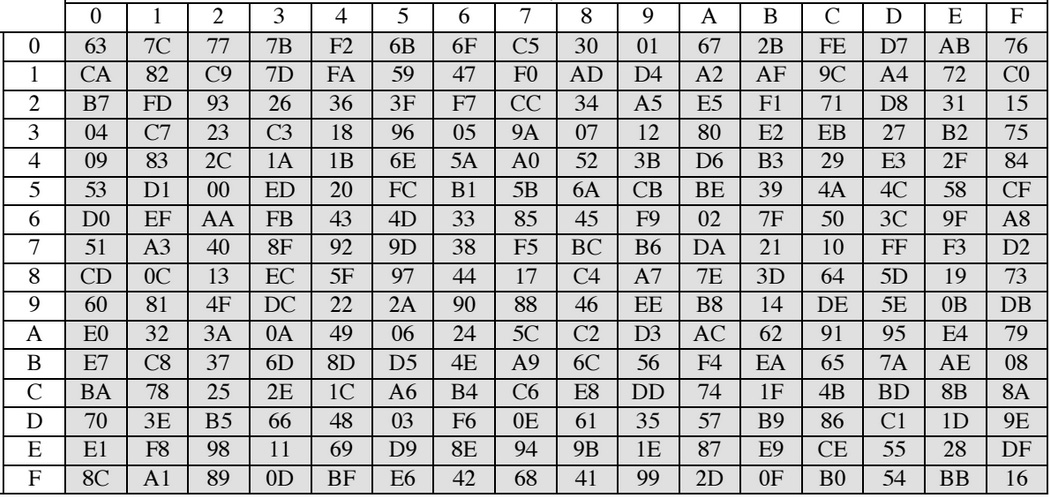
\includegraphics[width=\textwidth]{imagens/aes-subbyte.jpg}
  \caption{Tabela SubByte precomputada.}
  \label{fig:subbyte}
\end{figure}

Na fase de descriptografia do AES outra matriz e outra constante são aplicadas e em seguida é calculado o inverso em GF($2^8$) de forma a reverter o processo.

Na fase {\em MixColumn} são selecionados quatro bytes que são dispostos em um vetor para ser multiplicado por uma matriz, cada passo da multiplicação é calculado em $GF(2^8)$.


\begin{example}
  Considere que os bytes $B_0, B_5, B_{10}$ e $B_{15}$ foram selecionados.
  Fazemos a seguinte conta:

\begin{displaymath}
\left(\begin{array}{cccc}
02_{16} & 03_{16} & 01_{16} & 01_{16} \\
01_{16} & 02_{16} & 03_{16} & 01_{16} \\
01_{16} & 01_{16} & 02_{16} & 03_{16} \\
03_{16} & 01_{16} & 01_{16} & 02_{16} \\
\end{array} \right) 
\left( \begin{array}{c}
B_0\\ B_5\\ B_{10}\\ B_{15}\\\end{array} \right)
=
\left( \begin{array}{c}
C_0\\ C_1\\ C_2\\ C_3\\\end{array} \right)
\end{displaymath}  

Para facilitar as contas suponha que todos os bytes selecionados ($B_0, B_5, B_{10}$ e $B_{15}$)são $25_{16}$.
Neste caso precisamos calcular $02_{16} \cdot 25_{16}$ e $03 \cdot 25_{16}$:


\begin{eqnarray*}
  02_{16} \cdot 25_{16} & = & x(x^5 + x^2 + 1)\\
                      & = & x^6 + x^3 + x\\
  03_{16} \cdot 25_{16} & = & (x + 1)(x^5 + x^2 + 1)\\ 
                      & = & x^6 + x^5 + x^3 + x^2 + x + 1\\ 
\end{eqnarray*}

Neste caso, como todos $B_i$ são iguais, todos os $C_i$ também o são e são calculados da seguinte forma:

\begin{displaymath}
  \begin{array}{cccccccccc}
    01_{16} \cdot 25_{16} & = & & x^5 + & & & x^2 + & & 1\\
    01_{16} \cdot 25_{16} & = & & x^5 + & & & x^2 + & & 1\\
    02_{16} \cdot 25_{16} & = & x^6 + & & & x^3 + & & x & \\
    03_{16} \cdot 25_{16} & = & x^6 + & x^5 + & & x^3 + & x^2 + & x + & 1\\
    \hline
    C_i & = & & x^5 + & & & x^2 + &  & 1\\
  \end{array}
\end{displaymath}
\end{example}

No processo de descriptografia uma outra matriz é usada para calcular o {\em MixCloumn}, uma que reverte o que foi calculado neste passo.